\chapter{ Description of the model \label{ch:numero_uno}}
\section{An invitation to algebraic representation of cell boundaries}\label{sec:introSDFs}
The use of signed distance fields (SDFs) to model organic sufaces
is a time honoured graphical technique used, for example, by Pixar
Animation Studios to model hair in \textit{The Incredibles} 
(see \cite{petrovic2005volumetric}). The idea is to define a 
function which represents the closest distance from the query point
to a point on the surface of the object that is to be represented. 
If the query point is outside, the SDF is positive,
the SDF is zero on the surface and negative inside. SDFs can be 
rendered within traditional graphics pipelines (such as OpenGL or Vulkan)
using raymarching, a method that takes place within shader programs and 
is therefore meshless. The formulae defining SDFs for common 2D and 3D 
shapes are easy to find online, see \cite{key}. In this thesis,
we do not use signed distance fields based on the practical 
reason that their definitions usually involve square roots
which are slow to compute. We employ very similar formula
without the square roots, which yield the same level sets (in 2D)
but are fast to compute.
\\

To motivate the primary mechanism by which cells will undergo mitosis 
in this thesis, we consider a toy example in which the level sectios of the equations for
a pair of ellipses undergo a catastrophic topological change as one real parameter 
changes, namely the distance $d$ between their centers. We start by considering 
the equations for two ellipses which 
begin as coincident and move apart as the parameter $d$ becomes larger. 
The equations that represent the individual cells are
\begin{equation*}
    f_1(x,y,z) = \left( \frac{x+d}{p} \right)^2 + \left( \frac{y}{q} \right)^2 - 1,
\end{equation*}
\begin{equation*}
    f_2(x,y,z) = \left( \frac{x-d}{p} \right)^2 + \left( \frac{y}{q} \right)^2 - 1,
\end{equation*}
where $p=1.0 L_0$ and $q=0.9 L_0$ are the semi-major radius and semi-minor radius
of the ellipses, respectively, 
and $d$ is the distance bewteen their centers. The aspect ratio is $q/p = 0.9$ and $L_0 = 7.5 \ \mu m$
is the average length of a  saccharomyces cerevisiae (Baker's yeast) cell in ideal conditions as per
\cite{chavez2024cell}.
\\

In order to generate 
the combined algebraic curve for the pair, which, by an abuse of notation, will 
be called the colony SDF from now on, we build the following.
This is done using a what is called a ``union" in computer graphics
(see \cite{fusekvisualization}). This is simply the pointwise minimum,
\begin{equation*}
    f_{\textrm{union}}(x,y,z) = \min(f_1(x,y,z), f_2(x,y,z)).
\end{equation*} 
To get a smooth transition between the cells as they come apart we could alternatively use 
the $\textrm{smoothmin}$ which is defined by a smoothness parameter $s$, as in
\begin{equation*}
    \textrm{smoothmin}(f_1(x,y,z), f_2(x,y,z); s) = -s \log(e^{-f_1(x,y,z)/s} + e^{-f_2(x,y,z)/s}).
\end{equation*}
\begin{figure}[!htb]
    \centering
    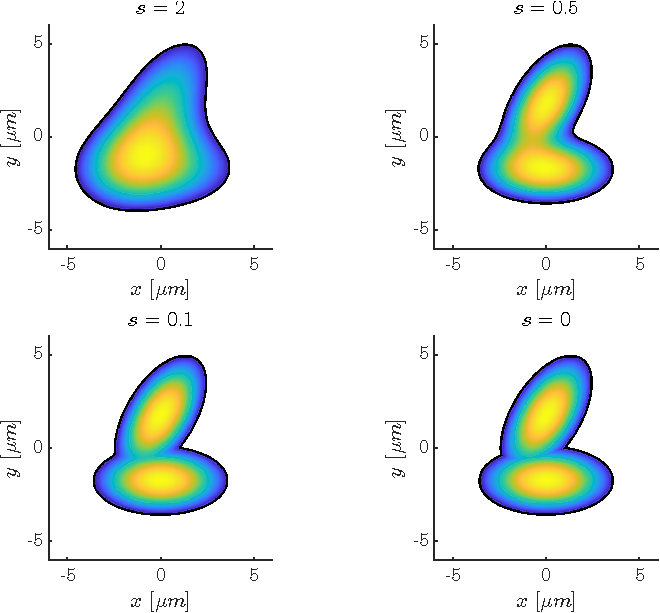
\includegraphics[width=0.8\textwidth]{chapter2/figures/compareSmoothness.pdf}
    \caption{Two ellipses blended with various values of smoothness $s$. The bottom right 
             figure is computed using standard minimum instead of smoothmin. Indeed,
             as $s \rightarrow 0$, the plot looks less smoothed across.}
    \label{fig:compareSmoothness}
\end{figure}
Figure \ref{fig:compareSmoothness} shows the effect of using different values of smoothness
$s$. Ultimately, using smoothmin was abandoned in favour or the computationally quicker \codeword{min},
which does not require the costly evaluation of the natural log and exponential functions.
\\

As shown in figure \ref{fig:mitosisplot}, we have a smooth splitting of a 
cell as the parameter $d$ ranges from $0.0$ to $9.1 \ \mu m$. Here $s$ is the 
smoothing parameter. In order to ensure that only the interior
of the SDF level section was plotted, I set positive entries to \codeword{nan},
which is MATLAB code for \textit{not a number}. The surface plots in figure \ref{fig:mitosisplot}
were produced via the use of MATLAB's \codeword{surf} function which ignores \codeword{nan} entries
in the underlying $Z$ matrix. One additional transformation made before plotting, was to multiply by 
$-1$ to reflect the SDF about the level plane, achieving a positive value inside the biomass.
\begin{figure}[!htb]
    \centering
    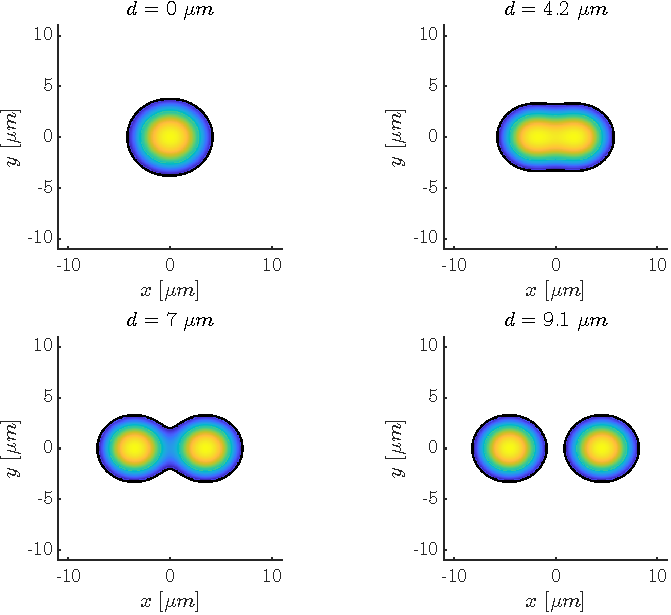
\includegraphics[width=0.8\textwidth]{chapter2/figures/mitosisPlot.pdf}
    \caption{The separation $d$ between two ellipse shapes with $s = 0.5$ and 
    an aspect ratio of $0.9$}
    \label{fig:mitosisplot}
\end{figure}
\\

A signed distance field for an ellipse is used to model Baker's yeast cells which
are in a pseudo-hyphal growth regime.
An ellipse centered at the origin with semi-major dimension $p$ (the $x$ intercept) and
semi-minor dimension $q$ (the $y$ intercept) has an SDF given by
\begin{equation*}
    f(x,y) = \sqrt{ \left( \frac{x}{p} \right)^2 + \left( \frac{y}{q} \right)^2 } - 1.
\end{equation*}
Recall that for computational efficiency we choose to use,
\begin{equation*}
    f(x,y) = \left( \frac{x}{p} \right)^2 + \left( \frac{y}{q} \right)^2  - 1.
\end{equation*}
This is not really a \textit{distance} field because it is 
dimensionless but it will still be called an SDF since it produces the 
elliptical shape all the same. We can also translate and rotate the ellipse, using
\begin{equation*} 
    \Delta \vb{x}' = 
    \begin{bmatrix}
        \cos{\theta} & \sin{\theta} \\
        -\sin{\theta} & \cos{\theta} 
    \end{bmatrix}
    \Delta \vb{x},
\end{equation*}
where $\Delta \vb{x} = (x-x_c) \hat{\vb{i}} + (y-y_c)\hat{\vb{j}} $ and $(x_c,y_c)$ is the
center of the ellipse. We call the components of $\Delta \vb{x} = \Delta x \hat{\vb{i}} +
\Delta y \hat{\vb{j}} $. The above trasnformation is a passive rotation because 
it rotates the whole SDF. The following equation
\begin{equation*}
    f(x,y) = \left[\frac{ (x-x_c)\cos{\theta} + (y-y_c) \sin{\theta}}{p} \right]^2 
        + \left[ \frac{-(x-x_c)\sin{\theta} +(y-y_c) \cos{\theta}}{q} \right]^2 - 1.
\end{equation*}
is used in the custom MATLAB function \codeword{ellipse.m} devloped here. Each individual 
cell has a unique value of $(x_c,y_c,p,q,\theta)$ which we index by $k$. Bringing them all 
together in one function using \codeword{min}, we have the colony SDF given by,
\begin{equation*}
    g(x,y) = \min_{k \in \{1, ..., N_{\textrm{cells}}\}} f_k(x,y),
\end{equation*}
where the individual SDF for each cell is given by 
\begin{equation*}
    \begin{split}
    f_k(x,y) &= \left[\frac{ (x-x_{c,k})\cos{\theta_k} + (y-y_{c,k}) \sin{\theta_k}}{p_k} \right]^2 \\ 
        &+ \left[ \frac{-(x-x_{c,k})\sin{\theta_k} +(y-y_{c,k}) \cos{\theta_k}}{q_k} \right]^2 - 1.
    \end{split}
\end{equation*}
Cell colonies can also be built up by combining the SDFs of the individual cells 
using a cumulative $\textrm{smoothmin}$.
\\

Some significant optimsations were made to make sure that the evalution of 
the colony SDF (evaluated via calling \codeword{ellipse.m}) was as fast as 
possible within the capabilities of MATLAB. These 
optimisations, which were crucial because \codeword{ellipse.m} is called per time step, 
are commented on in Chapter 2, subsection \ref{ssec:ellipse}.

\section{Cell colony dynamics with an underlying discrete network}
Now that we have introduced a robust mechanism to represent cell colony 
shape, the question naturally arises about how to represent the time dependence of this 
morphology. Baker's yeast grows via budding,
as shown in figure \ref{fig:yeastMicrograph}.
\begin{figure}[!htb]
    \centering
    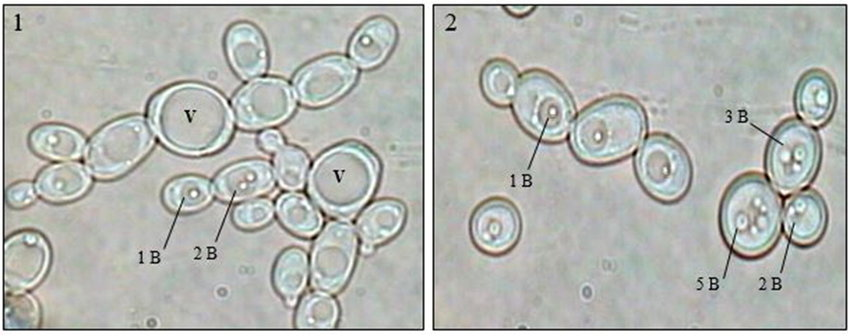
\includegraphics[width=0.8\textwidth]{chapter2/figures/yeastMicrograph.png}
    \caption{Micrographs of a translucent yeast strain studied
             in \cite{ebrahimi2020yeast}.}
    \label{fig:yeastMicrograph}
\end{figure}
To represent the branching dynamics of pseudo-hyphal yeast growth, 
an underlying discrete network which can change node count has been developed.
A colony for which the node count $N_{\textrm{nodes}}$ remains fixed is given 
by a undirected graph with adjacency matrix $A_{ij}$ where the edges are symbolically
represented by springs which model the elasticity of the cells. 
A diagram of this is shon in figure \ref{fig:yeastAsSpringNetwork}. 
\begin{figure}[!htb]
    \centering
    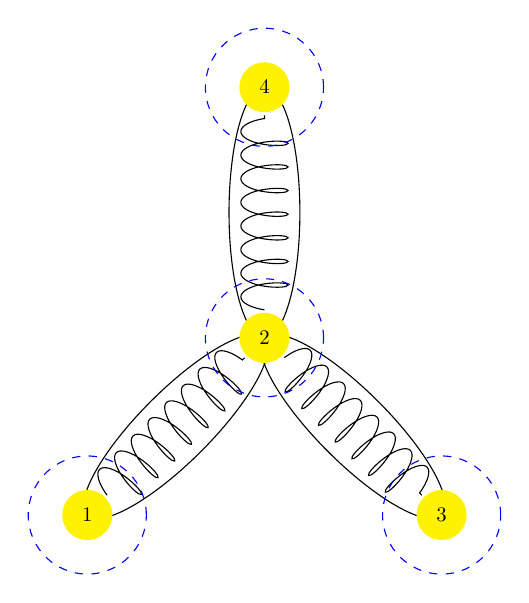
\begin{tikzpicture}
        \begin{scope}[scale=0.75,transform shape]
        \draw[rotate=45] (-0.5*4.243cm,0) ellipse (0.5*4.243cm and 0.6cm);
        \draw[rotate=-45] (0.5* 4.243,0) ellipse (0.5*4.243cm and 0.6cm);
        \draw[rotate=0] (0.0,0.5* 4.243)  ellipse (0.6cm and 0.5*4.243cm);
        
        \node[circle,fill=yellow, line width=1mm,inner sep=2.0mm] (a) at (-3,-3)  {1};
        \node[circle,fill=yellow, line width=1mm,inner sep=2.0mm] (b) at (0,  0)  {2};
        \node[circle,fill=yellow, line width=1mm,inner sep=2.0mm] (c) at (3, -3)  {3};
        \node[circle,fill=yellow, line width=1mm,inner sep=2.0mm] (d) at (0,4.243){4};
        \draw[decoration={aspect=0.3, segment length=3mm, amplitude=3mm,coil},decorate] (a) -- (b);
        \draw[decoration={aspect=0.3, segment length=3mm, amplitude=3mm,coil},decorate] (b) -- (c);  
        \draw[decoration={aspect=0.3, segment length=3mm, amplitude=3mm,coil},decorate] (b) -- (d); 

        \draw[dashed, color=blue]   (a)  ellipse (1.0cm and 1.0cm);
        \draw[dashed, color=blue]   (b)  ellipse (1.0cm and 1.0cm);
        \draw[dashed, color=blue]   (c)  ellipse (1.0cm and 1.0cm);
        \draw[dashed, color=blue]   (d)  ellipse (1.0cm and 1.0cm);
        \end{scope}
    \end{tikzpicture}
    
    \caption{A diagram of three elliptical cells with internal springs to represent biomass 
             elasticity ($\lambda_2 = \frac{K}{\eta \mu}$). The nodes are positioned at the ends of the major dimension
             of each ellipse and there are two nodes per cell. The force acting on 
             node $2$ for instance would be due to the forces from nodes $1$, $3$ and $4$.
             The dashed red circles represent the activation radius ($ \lambda_4 = R/L_0$) 
             of the contact force between the nodes.}
    \label{fig:yeastAsSpringNetwork}
\end{figure}

Relating the positions of the nodes in the network is done 
based on a simple implementation shown in figure \ref{fig:yeastMicrograph}.
\begin{figure}[!htb]
    \centering
    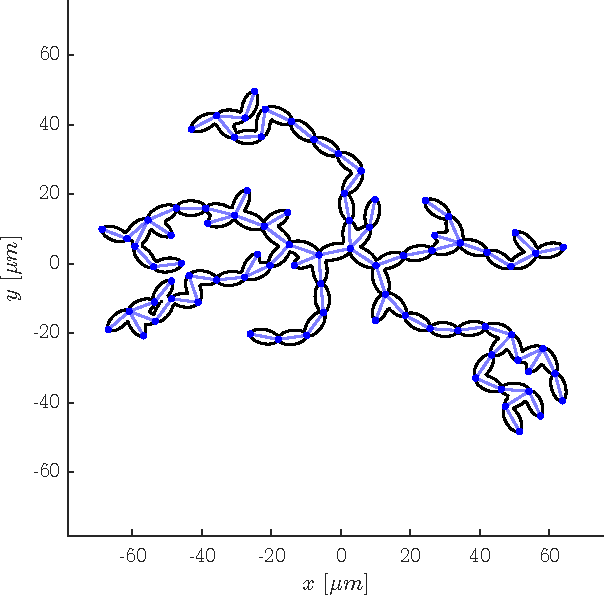
\includegraphics[width=0.6\textwidth]{chapter2/figures/networkYeast.pdf}
    \caption{A plot showing the underlying network of a simulated yeast colony 
            as well as the level-$0$ contour of the corresponding colony SDF.}
    \label{fig:yeastMicrograph}
\end{figure}
The equations that represent this correspondence between a cell indexed $k$ having 
parameters $(x_{c,k}, y_{c,k}, p_k, q_k, \theta_k)$
and its constitutive nodes indexed $i_1$ and $i_2$ are given by,
\begin{equation}
    p_k(t) = \frac{1}{2}||\vb{x}_{i_1} - \vb{x}_{i_2}||, \ 
    \textrm{where cell} \ k \ \textrm{is comprised of nodes} \ i_1, i_2, 
\end{equation}
\begin{equation}
    q_k(t) = \lambda_7 p_k(t), 
\end{equation}
\begin{equation}
    \theta_k(t) = \atan (y_{i_1} - y_{i_2},x_{i_1} - x_{i_2} ), 
\end{equation}
\begin{equation}
    \vb{x}_{c,k}(t) = \frac{1}{2} \left(\vb{x}_{i_1}(t) + \vb{x}_{i_2}(t)\right),
\end{equation}
where $\atan$ is the $2$ argument inverse tangent. In table \ref{table:perCellVariables} the variables 
associated with the cell indexed $k$, comprised of nodes $i_1$ and $i_2$ are summarised.

\begin{table}[!htb]
\begin{center}
    \begin{tabular}{ |c|c|c| } 
     \hline
      \textbf{Symbol} & \textbf{Formula in terms of nodes $i_1, i_2$} & \textbf{Description} \\ 
      \hline
     $\vb{x}_{c,k}$ & $\frac{1}{2} \left(\vb{x}_{i_1} + \vb{x}_{i_2}\right)$     & Center \\ 
     $p_k$          & $\frac{1}{2}||\vb{x}_{i_1} - \vb{x}_{i_2}||$                     & Semi-major radius \\ 
     $q_k$          & $\frac{\lambda_7}{2}||\vb{x}_{i_1} - \vb{x}_{i_2}||$                                      & Semi-minor radius \\         
     $\theta_k$     & $\atan (y_{i_1} - y_{i_2},x_{i_1} - x_{i_2} )$                   & Orintation angle \\         
     \hline   
    \end{tabular}   
\end{center}
\caption{The variables associated with each cell indexed $k$ and comprised of 
         nodes $i_1$ and $i_2$.}
\label{table:perCellVariables}
\end{table}

\section{The colony adjacency matrix, $A$}
In the software \codeword{CellColonySimulator} developed, the maximum 
number of nodes which the simulation can take is set to 
\codeword{maxNodeCount = 500}. This number is of course arbitrary and 
can be chosen to be much larger if the supercomputing time is available. 
In the case of figure \ref{fig:yeastAsSpringNetwork}, suppose
\codeword{maxNodeCount = 5}. Since there are only $4$ active nodes,
we would have an adjacency matrix of 
\begin{equation*}
    A = 
    \begin{bmatrix}
    0 & 1 & 0 & 0 & 0  \\
    1 & 0 & 1 & 1 & 0  \\
    0 & 1 & 0 & 0 & 0  \\
    0 & 1 & 0 & 0 & 0  \\
    0 & 0 & 0 & 0 & 0  \\ 
    \end{bmatrix},
\end{equation*}
which encodes the connectivity, i.e. node $1$ is connected to node $2$ and so on.
In order to represent the spring force from nodes $1$, $3$ and $4$ acting on node $2$,
we would sum up the spring forces from each connected node and apply Newton's Second Law, 
in the overdamped regime
\begin{equation*}
    \vb{v}_2 = \frac{\vb{F}_2}{\eta},
\end{equation*}
where $\vb{v}_2$ is the node 2's velocity, $\vb{F}_2$ is the net force acting on 
node 2, and $\eta$ is the dampening constant which is assumed to be uniform in the simulation.
The force on node 2 due to node 1 for example is given by $\vb{F}_{21}$ as 
\begin{equation*}
    \vb{F}_{21} = -K \left( ||\vb{x}_2 - \vb{x}_1|| - L_0 \right) \frac{\vb{x}_2 - \vb{x}_1}{||\vb{x}_2 - \vb{x}_1||},
\end{equation*}
which is Hooke's Law for a spring of stiffness $K$ and nominal length $L_0$.
The force acting on node 2 then is,
\begin{equation*}
    \vb{F}_{2} = \vb{F}_{21} + \vb{F}_{23} + \vb{F}_{24},
\end{equation*}
where the forces $\vb{F}_{23}$ and $\vb{F}_{24}$ are similarly defined. For a
system of nodes with arbitrary connectivty, the net force 
acting on node $i$ is given by 
\begin{equation*}
    \vb{F}_{i} = \sum_{j = 1, j \neq i}^{N_{\textrm{nodes}}} A_{ij} \vb{F}_{ij},
\end{equation*}
where $\vb{F}_{ij}$ is the spring force on node $i$ due to node $j$.
\\

In a very similar way, we add in a constant contact force between the nodes with radius $R \leq \frac{1}{2}L_0$,
which ensures that the nodes do not overlap. This is sometimes called an exclusion principle. The third 
type of force is in a sense an external driving force for the colony. It is a force 
proportional to the nutrient concentration gradient $\nabla c(\vb{x}_i, t)$ at the cell position. This type of 
force represents the attraction of the cells to areas of the petri dish with a high nutrient concentration.
A separate equation for the nutrient dynamics is introduced in section \ref{sec:nutrientField}. 
All of the three types of forces: elastic, contact and chemotaxis are added together to 
determine the motion of each node.
\begin{equation} \label{eqn:forcesNode_i}
    \begin{split}
        \frac{d \vb{x}_i}{dt} &= 
        \frac{K}{ \eta}\sum_{j = 1, j \neq i}^{N_{\textrm{nodes}}}   \left[ - A_{ij} \left( ||\vb{x}_i - \vb{x}_j|| - L_0\right) \frac{\vb{x}_i - \vb{x}_j}{||\vb{x}_i - \vb{x}_j||} \right]\\
         &+ \frac{F}{ \eta}\sum_{j = 1, j \neq i}^{N_{\textrm{nodes}}} \left[ H(R - ||\vb{x}_i - \vb{x}_j||) \frac{\vb{x}_i - \vb{x}_j}{||\vb{x}_i - \vb{x}_j||}     \right]\\ 
         &+ \frac{\gamma}{\eta} \nabla c (\vb{x}_i, t),
    \end{split}
\end{equation}
where $F$ is the magnitude of the contact force, and $\gamma$ is the magnitude of chemotaxis. In equation 
\ref{eqn:forcesNode_i} we have used the kinematic relationship $\vb{v}_i = \frac{d \vb{x}_i}{dt}$ and 
$H$ denotes a step function which is $0$ for a negative argument and $1$ for an arguemnt in 
$\mathbb{R}_{\geq 0}$.



\section{New cells from old}
We add in nodes at a small distance $\delta = 0.01$ beside old nodes 
which are taken to be parent nodes. The addition of new nodes is done in global mitosis events 
at time indices $n$ that are a multiple of
\begin{equation*}
    \Delta n = \bigg\lceil \frac{1}{\Delta t} \bigg\rceil,
\end{equation*}
where $\Delta t$ is the (non-dminesionalised) simulation time step, taken to be $0.01$ in \\
 \codeword{CellColonySimulator}.
The number of cells added at each global mitosis event reflects the exponential growth equation,
\begin{equation*}
    N_{\textrm{nodes}} = N_{0, \textrm{cell}} e^{t \mu(t)},
\end{equation*}
where the time-dependent growth rate $\mu$ is discussed 
in more detail in Chapter 2, subsection \ref{ssec:runSimulation}. The growth rate 
itself is given to be proportional to the average nutrient concentration over the node indices, and 
is given by equation \ref{eqn:growthRate}. This reflects the fact that if the nutrient has been depleted,
no new cells should be added, whereas if the nutrient has a uniform concentration of $1.0 \ \mu m^{-2}$ 
(taken to be the ideal nutrient concentration for growth and explained in section \ref{sec:nonDimEOMs}), 
then the colony will grow at the ideal growth rate, given by $\mu^*$.
\\

\begin{figure}[!htb]
    \centering
    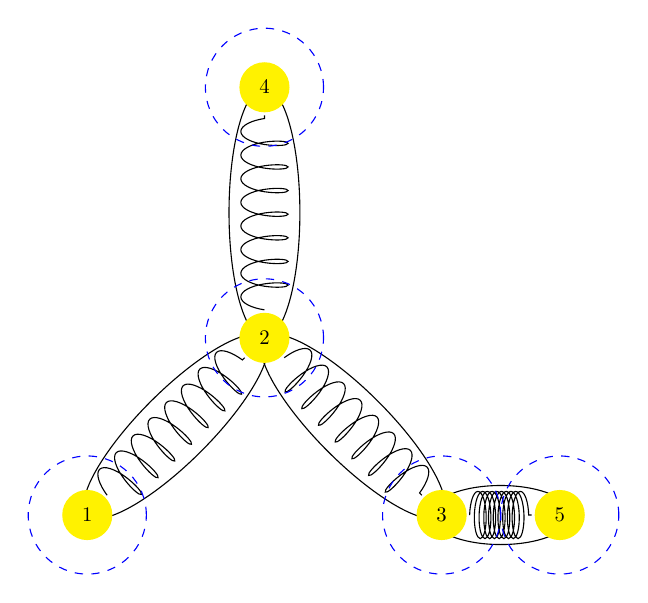
\begin{tikzpicture}
        \begin{scope}[scale=0.75,transform shape]
        \draw[rotate=45] (-0.5*4.243cm,0) ellipse (0.5*4.243cm and 0.6cm);
        \draw[rotate=-45] (0.5* 4.243,0) ellipse (0.5*4.243cm and 0.6cm);
        \draw[rotate=0] (0.0,0.5* 4.243)  ellipse (0.6cm and 0.5*4.243cm);
        \draw[rotate=0] (4.0,-3.0)  ellipse (1.2cm and 0.5cm);

        \node[circle,fill=yellow, line width=1mm,inner sep=2.0mm] (a) at (-3,-3)  {1};
        \node[circle,fill=yellow, line width=1mm,inner sep=2.0mm] (b) at (0,  0)  {2};
        \node[circle,fill=yellow, line width=1mm,inner sep=2.0mm] (c) at (3, -3)  {3};
        \node[circle,fill=yellow, line width=1mm,inner sep=2.0mm] (d) at (0,4.243){4};
        \node[circle,fill=yellow, line width=1mm,inner sep=2.0mm] (e) at (5,-3){5};
        \draw[decoration={aspect=0.3, segment length=3mm, amplitude=3mm,coil},decorate] (a) -- (b);
        \draw[decoration={aspect=0.3, segment length=3mm, amplitude=3mm,coil},decorate] (b) -- (c);  
        \draw[decoration={aspect=0.3, segment length=3mm, amplitude=3mm,coil},decorate] (b) -- (d); 
        \draw[decoration={aspect=0.3, segment length=0.6mm, amplitude=3mm,coil},decorate] (c) -- (e); 

        \draw[dashed, color=blue]   (a)  ellipse (1.0cm and 1.0cm);
        \draw[dashed, color=blue]   (b)  ellipse (1.0cm and 1.0cm);
        \draw[dashed, color=blue]   (c)  ellipse (1.0cm and 1.0cm);
        \draw[dashed, color=blue]   (d)  ellipse (1.0cm and 1.0cm);
        \draw[dashed, color=blue]   (e)  ellipse (1.0cm and 1.0cm);
        \end{scope}
    \end{tikzpicture}
    \caption{A mitosis event occurs via the addition of new nodes connected to old nodes.
             The nodes are added very close (distance $\delta \ll 1$) by the original nodes (exaggerated here)
             so that the spring force can be defined. After this point, 
             the initially compressed cell ``grows" outwards to achieve its nominal length, under 
             the influence of elasticity, contact and chemotactic forces.}
    \label{fig:addingACell}
\end{figure}
Figure \ref{fig:addingACell}, demonstrates the mechanism by which a new node is added to the 
colony, in this case, node $5$. The colony connectivity of this new $5$-node network would be given as 
\begin{equation*}
    A' = 
    \begin{bmatrix}
    0 & 1 & 0 & 0 & 0  \\
    1 & 0 & 1 & 1 & 0  \\
    0 & 1 & 0 & 0 & 1  \\
    0 & 1 & 0 & 0 & 0  \\
    0 & 0 & 1 & 0 & 0  \\ 
    \end{bmatrix},
\end{equation*}
because node $5$ is connected to node $3$. We mention that the new colony 
is defined by a different equilibrium position (when the time-derivative of 
position is quasi-steady).



\section{Incorporating the nutrient field} \label{sec:nutrientField}
A nutrient medium containing glucose is assumed to be given by a reaction-diffusion 
partial differential equation. That is the nutrient concentration $c(x,y,t)$ is given by
\begin{equation*}
    \pdv{c(x,y,t)}{t} = D \left( \frac{\partial^2 c(x,y,t)}{\partial x^2} + 
                          \frac{\partial^2 c(x,y,t)}{\partial y^2} \right) - r c(x,y,t) b(x,y,t)
\end{equation*}
where $b(x,y,t)$ is the microscopic biomass density of the cell colony, $D$ is a diffusion
coefficient and $r$ is a constant measuring the rate at which the cells consume nutrient.
The biomass field $b(x,y,t)$ is given as a function of the colony SDF as,
\begin{equation*}
    b(x,y,t) = \begin{cases}
                -g(x,y,t), & \ \textrm{if} \ g(x,y,t) \leq 0, \\
                0,         & \ \textrm{otherwise}.
               \end{cases}
\end{equation*}
In the case of the plotting of $b(x,y,t)$ we use \codeword{nan} instead of $0$. 
\\

The PDE is subjected to the Dirichlet condition
that the nutrient density takes a value of $1.0$ at the boundary. In order to simulate the nutrient field
numerically a foward time centered space (FTCS) scheme was prototyped on the square grid 
covering the domain. However, this scheme was found to be numerically unstable
for small spatial steps $h$ and large time steps $\Delta t$ and was discarded
in favour of the unconditionally numerically stable Crank-Nicholson scheme detailed
in section \ref{Crank_Nicholson}. Before this is possible, 
we carry out the non-dimensionalising of the equations of motion (EOMs).


\section{Non-dimensionalising the equations of motion}\label{sec:nonDimEOMs}

In order to non-dimensionalise the equations of motion (EOMs) we
introduce dimensionless parameters $\vb{x}_i = X\hat{\vb{x}}_i$, $t = T \hat{t}$, $b = B \hat{b}$
and $c = G \hat{c}$, where $X, T, B$ and $G$ are general undetermined scalings for the independent 
and dependent variables, respectively. At the outset, we fix $X = L_0 = 7.5 \ \mu m$ the nominal major cell diameter
found by \cite{chavez2024cell}. The same source gives an aspect ratio
of $7.5 \times 5.5 \ \mu m$ which we call $\lambda_7 = \frac{q}{p}$. The reason for the numbering 
will become clear from the non-dimensionalisation of the model. The time scale is chosen as
$T = \frac{1}{\mu^*}$ the reciprocal of specific growth rate for yeast, that is the $\mu^* = \mu(0)$ that appears in
the formula for the total node count. The value chosen was $\mu^* = 0.46$ hour$^{-1}$
from the value cited at \cite{salari2017investigation} which represents ideal conditions
for saccharomyces cerevisiae growth on a synthetic culture medium containing glucose. 
The value given by (\cite{salari2017investigation}) is a doubling rate of $90$ mins. In the model
presented in this thesis, that amounted to $\mu^* = \frac{\log(2)}{1.5 \ \textrm{hours}} = 0.4621$ hour$^{-1}$ which
was rounded down to $0.46$ hour$^{-1}$ as a conservative estimate.

\begin{table}[!htb]
\begin{center}
    \begin{tabular}{ |c|c|c| } 
     \hline
      \textbf{Symbol} & \textbf{Value} & \textbf{Descriptive name} \\ 
      \hline
     $L_0$   & $7.5 \ \mu m$       & Average cell length \\ 
     $\mu^*$ & $0.46$ hour$^{-1}$   & Ideal growth rate  \\ 
     $c_0$   & $1.0 \ \mu m^{-2}$  & Nutrient concentration \\ 
     \hline
     
    \end{tabular}
    
\end{center}
\caption{A summary of the numerical units}
\label{table:NumericalUnits}
\end{table}

It is necessary to point out that initial concentration, the choice for $G = c_0$, is 
typically measured in mol$\cdot \mu m^{-2}$ which amounts to Avagadro's number of 
glucose molecules per $\mu m^{2}$. In our case, we choose a number $N_G$ such that 
the concentration comes out to $1.0 \ N_G \cdot \mu m^{-2}$. We always
omit the $N_G$ because it is of no consequence dimensionally.
Also useful to recapitulate, is the formula for the total node count,
\begin{equation}  
    N_{\textrm{nodes}}(t) = N_{\textrm{cells},0} e^{ t \mu^* \hat{\mu}(t)},
\end{equation}
where $N_{\textrm{cells},0} = 1$ because we always begin with a single cell,
and $\hat{\mu}(t)$ is the unitless growth rate. Note that
$\mu(t) = \mu^* \hat{\mu}(t)$ and that $\hat{\mu}(0) = 1.0$.
This equation is used in the computation of $\mu^*$ based on the doubling time
provided in \cite{salari2017investigation}.
Hopefully it is clear that
the values of $L_0, \mu^*, c_0$
can be changed to fit different species of fungus. Those values given here
are just representative and further controlled experimental studies would 
need to be done to verify them.

\subsection{Non-dimensionalising the nutrient PDE}

Substituting these parameters into the reaction-diffusion PDE for nutrient concentration, we obtain 
\begin{equation*}
    \frac{c_0}{(1/\mu^*)}\pdv{\hat{c}}{\hat{t}} = \left(\frac{D c_0}{ L_0^2} \right)\left(\pdv[2]{\hat{c}}{\hat{x}} + \pdv[2]{\hat{c}}{\hat{y}} \right) -
      \left( r c_0 B\right)  \hat{c}\hat{b},
\end{equation*}
which results in 
\begin{equation*}
    \pdv{\hat{c}}{\hat{t}} = \left(\frac{D}{ \mu^* L_0^2} \right)\left(\pdv[2]{\hat{c}}{\hat{x}} + \pdv[2]{\hat{c}}{\hat{y}} \right) -
      \left( \frac{r  B}{\mu^*}\right)  \hat{c}\hat{b}.
\end{equation*}
Call the dimensionless diffusion constant $\lambda_1 = \frac{D}{ \mu^* L_0^2}$ and 
set $\frac{r  B}{\mu^*}=1$ which are free to do since $B$ is unset to begin with. This means 
that the scaling for the biomass density is $B = \frac{\mu^*}{r}$. The reaction diffusion equation 
reduces to 
\begin{equation*}
    \pdv{\hat{c}}{\hat{t}} = \lambda_1 \left(\pdv[2]{\hat{c}}{\hat{x}} + \pdv[2]{\hat{c}}{\hat{y}} \right) -
      \hat{c}\hat{b}.
\end{equation*}

\subsection{Non-dimensionalising the nodes ODE}
Now, for the EOM for the nodes, we have
\begin{equation*}
    \begin{split}
        \frac{d \vb{x}_i}{dt} &= 
        \frac{K}{ \eta}\sum_{j = 1}^N   \left[ - A_{ij} \left( ||\vb{x}_i - \vb{x}_j|| - L_0\right) \frac{\vb{x}_i - \vb{x}_j}{||\vb{x}_i - \vb{x}_j||} \right]\\
         &+ \frac{F}{ \eta}\sum_{j = 1}^N \left[ H(R - ||\vb{x}_i - \vb{x}_j||) \frac{\vb{x}_i - \vb{x}_j}{||\vb{x}_i - \vb{x}_j||}     \right]\\ 
         &+ \frac{\gamma}{\eta} \nabla c (\vb{x}_i, t).
    \end{split}
\end{equation*}
Substituting the dimensionless parameters, we acquire
\begin{equation*}
    \begin{split}
        \frac{L_0}{(1/\mu^*)}\frac{d \hat{\vb{x}}_i}{d \hat{t}} &= 
        \frac{K L_0}{ \eta}\sum_{j = 1, j \neq i}^N   \left[ - A_{ij}\left( ||\hat{\vb{x}}_i - \hat{\vb{x}}_j|| -  1\right) \frac{\hat{\vb{x}}_i - \hat{\vb{x}}_j}{||\hat{\vb{x}}_i - \hat{\vb{x}}_j||} \right]\\
         &+ \frac{F}{  \eta}\sum_{j = 1, j \neq i}^N \left[H(\hat{R} - ||\hat{\vb{x}}_i - \hat{\vb{x}}_j||) \frac{\hat{\vb{x}}_i - \hat{\vb{x}}_j}{||\hat{\vb{x}}_i - \hat{\vb{x}}_j||}     \right]\\ 
         &+ \frac{\gamma C}{ \eta L_0} \hat{\nabla}  \hat{c} (\hat{\vb{x}}_i, \hat{t}),
    \end{split}
\end{equation*}
which, after rearranging, becomes,
\begin{equation*}
    \begin{split}
        \frac{d \hat{\vb{x}}_i}{d \hat{t}} &= 
        \frac{K}{ \eta \mu^*}\sum_{j = 1, j \neq i}^N   \left[ - A_{ij}\left( ||\hat{\vb{x}}_i - \hat{\vb{x}}_j|| -  1\right) \frac{\hat{\vb{x}}_i - \hat{\vb{x}}_j}{||\hat{\vb{x}}_i - \hat{\vb{x}}_j||} \right]\\
         &+ \frac{F}{  \eta \mu^* L_0}\sum_{j = 1, j \neq i}^N \left[H(\hat{R} - ||\hat{\vb{x}}_i - \hat{\vb{x}}_j||) \frac{\hat{\vb{x}}_i - \hat{\vb{x}}_j}{||\hat{\vb{x}}_i - \hat{\vb{x}}_j||}     \right]\\ 
         &+ \frac{\gamma C}{ \eta \mu^* L_0^2} \hat{\nabla}  \hat{c} (\hat{\vb{x}}_i, \hat{t}).
    \end{split}
\end{equation*}
Only one of the coefficients could be set to unity, but instead we choose $C = c_0 = 1$ to be the initial 
concentration. That leaves us with four additional parameters,
\begin{equation*}
    \lambda_2 = \frac{K}{ \eta \mu^*},
\end{equation*}
\begin{equation*}
    \lambda_3 = \frac{F}{  \eta \mu^* L_0},
\end{equation*}
\begin{equation*}
    \lambda_4 = \frac{R}{L_0},
\end{equation*}
\begin{equation*}
    \lambda_5 = \frac{\gamma c_0}{ \eta \mu^*L_0^2}.
\end{equation*}

\subsection{Non-dimensionalising the biomass equation}
The field $g(x,y,t) = \hat{g}(\hat{x},\hat{y},\hat{t})$ is unitless 
so we are left with the following EOM for the biomass field,
\begin{equation*}
    B\hat{b} = \begin{cases}
                -  \hat{g}(\hat{x},\hat{y},\hat{t}), & \ \textrm{if} \ \hat{g}(\hat{x},\hat{y},\hat{t}) \leq 0, \\
                    0, &    \ \textrm{otherwise}.
               \end{cases}
\end{equation*}
\begin{equation*}
    \hat{b} = \begin{cases}
                -  \frac{r}{\mu^*}\hat{g}(\hat{x},\hat{y},\hat{t}), & \ \textrm{if} \ \hat{g}(\hat{x},\hat{y},\hat{t}) \leq 0, \\
                    0, &    \ \textrm{otherwise}.
               \end{cases}
\end{equation*}
which leaves us with an additional parameter, $\lambda_6 =\frac{r}{\mu^*}$. The final model parameter is the cell aspect ratio, $\lambda_7$.
The model parameters are summarised in table \ref{table:VariableNames}.


\begin{table}[!htb]
\begin{center}
    \begin{tabular}{ |c|c|c| } 
     \hline
      \textbf{Symbol} & \textbf{Expression} & \textbf{Descriptive name} \\ 
      \hline
     $\lambda_1$ & $\frac{D}{ \mu^* L_0^2}$ & diffusivity \\ 
     $\lambda_2$ & $\frac{K}{ \eta \mu^*}$ & elasticity \\ 
     $\lambda_3$ & $\frac{F}{  \eta \mu^* L_0}$ & respulsivity \\ 
     $\lambda_4$ & $\frac{R}{L_0}$ & respulsion radius \\ 
     $\lambda_5$ & $\frac{\gamma c_0}{ \eta \mu^* L_0^2}$ & mobility \\ 
     $\lambda_6$ & $\frac{r}{\mu^*}$ & metabolic rate \\ 
     $\lambda_7$ & $\frac{\textrm{cell minor axis}}{\textrm{cell major axis}} = \frac{2q}{2p}$ & cell aspect ratio \\ 
     \hline
     
    \end{tabular}
    
\end{center}
\caption{A summary of the dimensionless model parameters}
\label{table:VariableNames}
\end{table}


\subsection{Non-dimensional model equations of motion (EOMs)}

Dropping the hats on variable symbols, we arive at the final system equations of motion which
span from equation \ref{eqn:EOMs_PDE} to \ref{eqn:centerPos}.


\begin{equation} \label{eqn:EOMs_PDE}
    \boxed{\pdv{c}{t} = \lambda_1 \left(\pdv[2]{c}{x} + \pdv[2]{c}{y} \right) - bc,
     \ \textrm{for} \ (x,y) \in \Omega \setminus \partial \Omega,}
\end{equation}
\begin{equation}
    \boxed{c(x,y,t) = 1.0, \ \textrm{for} \ (x,y) \in \partial \Omega,}
\end{equation}
\begin{equation}
    \boxed{c(x,y,0) = 1.0,}
\end{equation}
\begin{equation}\label{eqn:EOMs_ODE}
    \boxed{
    \begin{split}
        \frac{d \vb{x}_i}{d t} 
         &= \lambda_2 \sum_{j=1}^{N_{\textrm{nodes}}} \left[ A_{ij}\left( 1- ||\vb{x}_i - \vb{x}_j|| \right) \frac{\vb{x}_i - \vb{x}_j}{||\vb{x}_i - \vb{x}_j||} \right]\\
         &+ \lambda_3 \sum_{j=1}^{N_{\textrm{nodes}}} \left[H(\lambda_4 - ||\vb{x}_i - \vb{x}_j||) \frac{\vb{x}_i - \vb{x}_j}{||\vb{x}_i - \vb{x}_j||}     \right]\\ 
         &+ \lambda_5 \nabla c (\vb{x}_i, t), \ \textrm{for} \ i \in \{ 1, ...,N_{\textrm{nodes}} \},  
    \end{split}}
\end{equation}
\begin{equation}
    \boxed{\vb{x}_1(0) = (0.5 \cos{\Theta_e}, 0.5 \sin{\Theta_e}), \ \vb{x}_2(0) = (-0.5 \cos{\Theta_e}, -0.5 \sin{\Theta_e}), }
\end{equation}
\begin{equation} \label{eqn:expGrowth}
    \boxed{N_{\textrm{nodes}} = N_{0, \textrm{cells}} e^{t \mu(t)}, \textrm{where} \ N_{0, \textrm{cells}} = 1, }
\end{equation}
\begin{equation}\label{eqn:growthRate}
    \boxed{\mu(t) = \frac{1}{N_{\textrm{nodes}}}\sum_{i=1}^{N_{\textrm{nodes}}} c(\vb{x}_i, t), } 
\end{equation}
\begin{equation} \label{eqn:biomass}
    \boxed{
    b(x,y,t) = 
    \begin{cases}
        -\lambda_6 g(x,y,t), & \ \textrm{if} \ g(x,y,t) \leq 0, \\
            0, &    \ \textrm{otherwise},
    \end{cases}
    }
\end{equation}
\begin{equation}
    \boxed{
    g(x,y,t) = \min_{k \in \{  1, ..., N_{\textrm{cells}}\}} f_k (x,y,t),
    }
\end{equation}
\begin{equation}
    \boxed{
    \begin{split}
    f_k(x,y,t) &= \left[\frac{ (x-x_{c,k}(t))\cos{\theta_k} + (y-y_{c,k}(t)) \sin{\theta_k}}{p_k(t)} \right]^2 \\ 
               &+ \left[ \frac{-(x-x_{c,k}(t))\sin{\theta_k} +(y-y_{c,k}(t)) \cos{\theta_k}}{q_k(t)} \right]^2 - 1,
    \end{split}
    }
\end{equation}
\begin{equation}\label{eqn:semiMajorAxis}
    \boxed{p_k(t) = \frac{1}{2}||\vb{x}_{i_1} - \vb{x}_{i_2}||, \ 
    \textrm{where cell} \ k \ \textrm{is comprised of nodes} \ i_1, i_2,} 
\end{equation}
\begin{equation}\label{eqn:semiMinorAxis}
    \boxed{q_k(t) = \lambda_7 p_k(t), }
\end{equation}
\begin{equation}\label{eqn:orientationAngle}
    \boxed{\theta_k(t) = \atan (y_{i_1} - y_{i_2},x_{i_1} - x_{i_2} ), }
\end{equation}
\begin{equation} \label{eqn:centerPos}
    \boxed{ \vb{x}_{c,k}(t) = \frac{1}{2} \left(\vb{x}_{i_1}(t) + \vb{x}_{i_2}(t)\right). }
\end{equation}

Note that $i$ and $j$ index over node numbers, $k$ over cells, and $i_1$ and $i_2$ denote the nodes
that comprise cell $k$. Also note that $\Theta_e$, the orientation of the starting cell
is chosen to be different for each ensemble instance $e$. In fact,
this is chosen to be a uniform random number between $[0,2\pi]$ which
is unpdated in the loop over the ensemble in \codeword{Master.m} as part of the \textbf{CellColonySimulator}
MATLAB software.
Finally the petri-dish domain is given by 

\begin{equation}
    \boxed{\Omega = \left[-\frac{1}{2}L_{\textrm{petri-dish}},\frac{1}{2}L_{\textrm{petri-dish}} \right] \times
             \left[-\frac{1}{2}L_{\textrm{petri-dish}},\frac{1}{2}L_{\textrm{petri-dish}} \right] \subset \mathbb{R}^2,}
\end{equation}
where it is noted that $L_{\textrm{petri-dish}}$ is unitless.


\section{Numerically solving for the nutrient field} \label{Crank_Nicholson}
In order to advance the nutrient field in time, an efficient and stable numerical solver
was required. Because of the fact that the nutrient field $c(x,y,t)$ is coupled 
to the biomass field which is dependent on a discrete network that changes in connectivity and 
node count, it was necessary to implement the method in-house, as opposed to 
using a pre-existing MATLAB boundary value solver for instance. The Crank-Nicolson method (\cite{crank1947practical}) was 
chosen for the practical reason that it led to faster simulations overall since a larger
time step could be used as opposed to the explicit forward in time central in space (FTCS) scheme. This 
is a direct consequence of the fact that the (implicit) Crank-Nicholson scheme is unconditionally numerically 
stable. Let us begin by verifying this fact using the what is
known as Von Neumann stability analysis (\cite{charney1950numerical}).
\begin{figure}[!htb]
    \centering
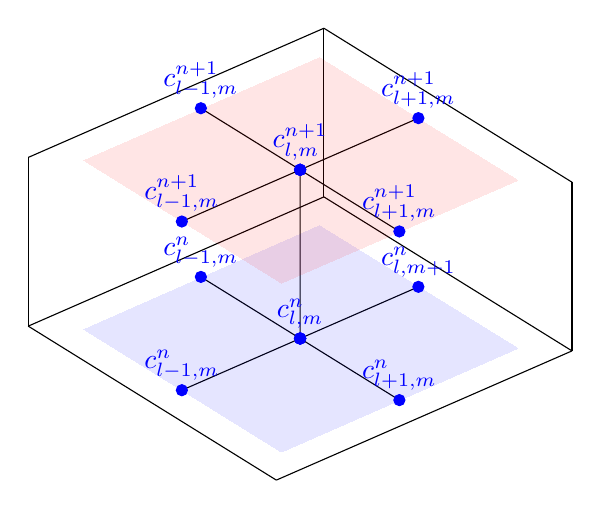
\begin{tikzpicture}
    \pgfplotsset{every tick label/.append style={font=\scriptsize}}
 
    \begin{axis}[view = {50}{50},
        width=0.7\textwidth,
        xmax = 10,
        xmin = -10,
        ymax = 10, 
        ymin = -10, 
        zmax = 10, 
        zmin = 0,
        xtick=\empty,
        ytick=\empty,
        ztick=\empty,
        grid,
        grid style={dashed,gray!40},
        3d box=background]
     
        \addplot3[mark=*,black,mark options={blue},point meta=explicit symbolic,nodes near coords] 
        coordinates 
        {
            (0,0,0) [$c_{l,m}^n$]
            (-8,0,0)[$c_{l-1,m}^n$]
            (0,0,0)
            (8,0,0)[$c_{l+1,m}^n$]
            (0,0,0)
            (0,8,0)[$c_{l,m+1}^n$]
            (0,0,0)
            (0,-8,0)[$c_{l-1,m}^n$]
            (0,0,0)
            (0,0,10)[$c_{l,m}^{n+1}$]
            (-8,0,10)[$c_{l-1,m}^{n+1}$]
            (0,0,10)
            (8,0,10)[$c_{l+1,m}^{n+1}$]
            (0,0,10)
            (0,8,10)[$c_{l+1,m}^{n+1}$]
            (0,0,10)
            (0,-8,10)[$c_{l-1,m}^{n+1}$]
        };

        \addplot3 [
        domain = -8:8,
        domain y = -8:8,
        samples = 2,
        samples y = 2,
        surf,
        fill opacity=0.1,
        shader = interp] {0};

        \addplot3 [
        domain = -8:8,
        domain y = -8:8,
        samples = 2,
        samples y = 2,
        surf,
        fill opacity=0.1,
        color=red,
        shader = interp] {10};
     
    \end{axis}
     
\end{tikzpicture}
\caption{The five point stencil for the nutrient field at times $t_{n} = n \Delta t$ (blue plane)
         and $t_{n+1} = (n+1) \Delta t$ (red plane) used for the Crank-Nicolson scheme on the domain
         interior.}
\label{fig:CrankNicolsonScheme}
\end{figure}

Firstly, we 
define the nutrient field as $c_{l,m}^{n} = c(x_l, y_m, t_n)$, where $x_l = -\frac{1}{2}L_{\textrm{petri-dish}} + h l$, 
$y_m = -\frac{1}{2}L_{\textrm{petri-dish}} + h m$ and similarly for $b_{l,m}^{n}$,
the biomass. The values  $c_{l,m}^{n}$ precisely satisfy the discretised equations which follow.
Let  $\bar{c}_{l,m}^{n}$ be the solution achieved with finite precison arithmetic 
operations which does not necessarily satisfy the equations, up to some error term,
\begin{equation*}
    \epsilon_{l,m}^n = \bar{c}_{l,m}^{n} - c_{l,m}^{n}.
\end{equation*}
Carrying out the Crank-Nicolson discretisation with the values $c_{l,m}^{n}$, we derive
\begin{equation*}
    \frac{c_{l,m}^{n+1} - c_{l,m}^{n}}{\Delta t} =
    \frac{\lambda_1}{2} \left( \nabla^2 c_{l,m}^{n+1} + \nabla^2 c_{l,m}^{n} \right) -
     \frac{1}{2} b_{l,m}^{n} (c_{l,m}^{n+1} + c_{l,m}^{n}).
\end{equation*}
The laplacian terms here are calculated with a five-point stencil at the current and subsequent 
time steps as shown in figure \ref{fig:CrankNicolsonScheme}. This results in the following discretisation,

\begin{equation*}
    \begin{split}
        \frac{c_{l,m}^{n+1} - c_{l,m}^{n}}{\Delta t} &=
        \frac{\lambda_1}{2}  \left( \frac{c_{l+1,m}^{n+1} - 2 c_{l,m}^{n+1} + c_{l-1,m}^{n+1} }{h^2} + 
                                    \frac{c_{l,m+1}^{n+1} - 2 c_{l,m}^{n+1} + c_{l,m-1}^{n+1} }{h^2} \right)  \\
                                   & +\frac{\lambda_1}{2} \left( \frac{c_{l+1,m}^{n} - 2 c_{l,m}^{n} + c_{l-1,m}^{n} }{h^2} + 
                                    \frac{c_{l,m+1}^{n} - 2 c_{l,m}^{n} + c_{l,m-1}^{n} }{h^2} \right) \\
                                   &-\frac{1}{2} b_{l,m}^{n} (c_{l,m}^{n+1} + c_{l,m}^{n}).
    \end{split}
\end{equation*}
To evaluate the numerical stability, we introduce a constant $\alpha = \frac{ \lambda_1 \Delta t }{h^2}$.
With this constant in place, we continue with
\begin{equation*}
    \begin{split}
        c_{l,m}^{n+1} - c_{l,m}^{n} &=
       \frac{\alpha}{2}  \left( c_{l+1,m}^{n+1} + c_{l-1,m}^{n+1} + 
                       c_{l,m+1}^{n+1} + c_{l,m-1}^{n+1}  \right) - 2 \alpha c_{j,k}^{n+1}  \\
                                   & +\frac{\alpha}{2} \left( c_{l+1,m}^{n}+ c_{l-1,m}^{n} + 
                                    c_{l,m+1}^{n} + c_{l,m-1}^{n}  \right) - 2 \alpha c_{l,m}^{n} \\
                                   &-\frac{\Delta t}{2} b_{l,m}^{n} (c_{l,m}^{n+1} + c_{l,m}^{n}).
    \end{split}
\end{equation*}
Since the discretised equations are linear in $c_{l,m}^{n}$ (taking $b_{l,m}^{n}$ to be slowly varying)
and since $\bar{c}_{l,m}^n$ also form a solution, the $\epsilon_{l,m}^n$ are also 
a solution.
\begin{equation*}
    \begin{split}
        \epsilon_{l,m}^{n+1} - \epsilon_{l,m}^{n} &=
       \frac{\alpha}{2}  \left( \epsilon_{l+1,m}^{n+1} + \epsilon_{l-1,m}^{n+1} + 
                                \epsilon_{l,m+1}^{n+1} + \epsilon_{l,m-1}^{n+1}  \right) - 2 \alpha \epsilon_{l,m}^{n+1}  \\
                                   & +\frac{\alpha}{2} \left( \epsilon_{l+1,m}^{n}+ \epsilon_{l-1,m}^{n} + 
                                   \epsilon_{l,m+1}^{n} + \epsilon_{l,m-1}^{n}  \right) - 2 \alpha \epsilon_{l,m}^{n} \\
                                   &-\frac{\Delta t}{2} b_{l,m}^{n} (\epsilon_{l,m}^{n+1} + \epsilon_{l,m}^{n}).
    \end{split}
\end{equation*}
We subsitute in an ansatz for the error term which is standard in Von Neumann stability analysis, namely
\begin{equation*}
    \epsilon_{l,m}^n = \xi^n e^{i \nu_x l h} e^{i \nu_y m h},
\end{equation*}
where $\nu_x$ and $\nu_y$ are wavenumbers and $h$ is the spatial step. Note that $i = \sqrt{-1}$. In order for the numerical
method to be stable, we require that $|\xi| \leq 1$ for all values of the wavenumbers $\nu_x, \nu_y$.
Substituting this expression into the discretised equation for the error, we get,
\begin{equation*}
    \begin{split}
        \xi^{n+1} e^{i \nu_x l h} e^{i \nu_y m h} - \xi^{n} e^{i \nu_x l h} e^{i \nu_y m h} &=
       \frac{\alpha}{2}  \left( \xi^{n+1} e^{i \nu_x (l+1) h} e^{i \nu_y m h} + \xi^{n+1} e^{i \nu_x (l-1) h} e^{i \nu_y m h} \right) \\
       &+ \frac{\alpha}{2}\left( \xi^{n+1} e^{i \nu_x l h} e^{i \nu_y (m+1) h} + \xi^{n+1} e^{i \nu_x l h} e^{i \nu_y (m-1) h}  \right) \\
       &-2 \alpha\xi^{n+1} e^{i \nu_x l h} e^{i \nu_y m h}  \\
       &+\frac{\alpha}{2} \left( \xi^{n} e^{i \nu_x (l+1) h} e^{i \nu_y k h}+ \xi^{n} e^{i \nu_x (m-1) h} e^{i \nu_y m h}\right) \\
       &+ \frac{\alpha}{2}\left(\xi^{n} e^{i \nu_x l h} e^{i \nu_y (k+1) h} + \xi^{n} e^{i \nu_x m h} e^{i \nu_y (m-1) h}  \right) \\
       &-2 \alpha \xi^{n} e^{i \nu_x l h} e^{i \nu_y k h}\\
       &-\frac{\Delta t}{2} b_{l,m}^{n} (\xi^{n+1} e^{i \nu_x l h} e^{i \nu_y m h} + \xi^{n} e^{i \nu_x l h} e^{i \nu_y m h}).
    \end{split}
\end{equation*}
Dividing through by $\xi^{n} e^{i \nu_x l h} e^{i \nu_y m h}$, we attain,
\begin{equation*}
    \begin{split}
        \xi - 1 &=
       \frac{\alpha}{2}  \left( \xi e^{i \nu_x h}+ \xi e^{-i \nu_x h} \right) 
       + \frac{\alpha}{2}\left( \xi  e^{i \nu_y h} + \xi  e^{-i \nu_y h}  \right) 
       -2 \xi \alpha  \\
       &+\frac{\alpha}{2} \left(  e^{i \nu_x  h}+  e^{-i \nu_x h}\right)
       + \frac{\alpha}{2}\left(   e^{i \nu_y h} +   e^{-i \nu_y  h}  \right) 
       -2 \alpha
       -\frac{\Delta t}{2} b_{l,m}^{n} (\xi + 1).
    \end{split}
\end{equation*}
Using the fact that $ \frac{e^{i \nu_x h}+  e^{-i \nu_x h}}{2} = \cos(\nu_x h)$ and similarly for
the other terms, we have,
\begin{equation*}
    \begin{split}
        \xi - 1 &=
         \alpha \xi \cos(\nu_x h) 
       + \alpha \xi \cos(\nu_y h) 
       -2 \alpha \xi   \\
       &+\alpha \cos(\nu_x h) 
       + \alpha \cos(\nu_y h) 
       -2 \alpha
       -\frac{\Delta t}{2} b_{l,m}^{n} (\xi + 1).
    \end{split}
\end{equation*}
Finally, solving for $\xi$, and taking its absolute value we have,
\begin{equation*}
    |\xi| = \left| \frac{1 + \alpha \left[ \cos(\nu_x h) + \cos(\nu_y h) \right] - 2 \alpha -\frac{1}{2} \Delta t b_{l,m}^{n} }
                        {1 -\alpha \left[ \cos(\nu_x h) + \cos(\nu_y h) \right]  + 2 \alpha +\frac{1}{2} \Delta t b_{l,m}^{n}} \right|.
\end{equation*}
In order to complete the analysis, consider when biomass is $b_{l,m}^{n} = 0$. We have the simplified
equation,
\begin{equation*}
    |\xi| = \left| \frac{1 -\alpha(2 - \left[ \cos(\nu_x h) + \cos(\nu_y h) \right]) }
                        {1 +\alpha(2 - \left[ \cos(\nu_x h) + \cos(\nu_y h)\right])} \right|,
\end{equation*}
Which has a numerator less than or equal to $1$ because $\alpha > 0$ and 
$0 \leq 2 - \left[ \cos(\nu_x h) + \cos(\nu_y h) \right] \leq 4$. The denominator is 
always greater than or equal to $1$, which is enough to prove that
the Crank-Nicolson scheme for the standard heat equation is numerically stable.
\\
\\
Whether this generalises to non-zero $b_{l,m}^{n}$ is determined by numerical experiments, and 
indeed for $\alpha = \frac{\lambda_1 \Delta t}{h^2} = \frac{(0.1) (0.01)}{(0.1)^2} = 0.1$, the scheme 
was not found to be unstable. However, for higher values of $\alpha$ it was possible to see spurious 
oscillations in the solution field for $c$ which obviously suggests some form of instability.





